\documentclass{beamer}

% You can also use a 16:9 aspect ratio:
%\documentclass[aspectratio=169]{beamer}
\usetheme{TACC16}

% It's possible to move the footer to the right:
%\usetheme[rightfooter]{TACC16}

%% page 
%\begin{frame}{}
%  \begin{itemize}
%    \item
%  \end{itemize}
%\end{frame}
%
%% page 
%\begin{frame}[fragile]
%    \frametitle{}
% {\tiny
%    \begin{semiverbatim}
%    \end{semiverbatim}
%}
%  \begin{itemize}
%    \item
%  \end{itemize}
%
%\end{frame}
 

\begin{document}
\title[Lmod]{SC 24 Booth Talk: Lmod}
\author{Robert McLay} 
\date{Nov. 20, 2024}

% page 1
\frame{\titlepage} 

\section{Introduction}

% page 2
\begin{frame}{Introduction}
  \center{\includegraphics[width=.9\textwidth]{Lmod-4color@2x.png}}
  \begin{itemize}
    \item Feature and Recent changes that bare repeating
    \item Changes in the pass year.
    \item Future work?
  \end{itemize}
\end{frame}

% page 3
\begin{frame}{Features}
  \begin{itemize}
    \item Current version is Lmod 8.7.53
    \item Release of 8.8 is very soon.
    \item Reads for TCL and Lua modulefiles
    \item One name rule.
    \item Support Software Hierarchy (but not required!)
    \item Spider Cache: fast \texttt{\color{blue} \$ module avail}
    \item Properties (gpu, beta. ...)
    \item family(``compiler'') family(``mpi'') support
    \item Optional Tracking: What modules are loaded?
    \item Many other features: ml, collections, hooks,
      extended default, nag ...
    \item Google analytics report about 2000 unique users around the
      world read docs every month.
  \end{itemize}
\end{frame}

% page 4
\begin{frame}{\texttt{Recent Feature of Lmod 8+}}
  \begin{itemize}
    \item The TCL interpreter is now (optionally) embedded with Lmod.
    \item \texttt{depends\_on()}
    \item New Function: \texttt{extensions("numpy/1.16.4 scipy/1.4")}
    \item Checking your module tree 8.4.3+
  \end{itemize}
\end{frame}

% page 5
\begin{frame}{\texttt{depends\_on()}}
  \begin{itemize}
    \item Modules X and Y depends on Module A
    \item ml purge; ml X; ml unload X;      $\Rightarrow$ unload A
    \item ml purge; ml X Y; ml unload X;    $\Rightarrow$ keep A
    \item ml purge; ml X Y; ml unload X Y ; $\Rightarrow$ unload A
    \item ml purge; ml A X Y; ml unload X Y ; $\Rightarrow$ keep A
  \end{itemize}
\end{frame}

% page 6
\begin{frame}{Checking your module tree 8.4.3+}
  \begin{itemize}
    \item New command added: \texttt{\$LMOD\_DIR/check\_module\_tree\_syntax}
    \item Reports syntax errors across the entire \texttt{\$MODULEPATH}
    \item Report which modules have multiple marked defaults sets
    \item Precedent order: default symlink, .modulerc.lua, .modulerc, .version
    \item Does not check SYSTEM MODULERCFILE for defaults.
  \end{itemize}
\end{frame}

% page 7
\begin{frame}{Lmod Recent Features}
  \begin{itemize}
    \item New Features now reported:
      https://lmod.readthedocs.io/en/latest/025\_new.html
    \item \texttt{module overview}
    \item \texttt{module -d avail}
    \item New config file: /etc/lmod/lmod\_config.lua
    \item LMOD\_QUARANTINE\_VARS
    \item updates to sh\_to\_modulefile
    \item source\_sh(): source a shell script inside a modulefile
  \end{itemize}
\end{frame}

% page 8
\begin{frame}[fragile]
  \frametitle{module overview}
    {\tiny
\begin{semiverbatim}
% module overview
------------------ /opt/apps/modulefiles/Core -----------------
StdEnv    (1)   hashrf    (2)   papi        (2)   xalt     (1)
ddt       (1)   intel     (2)   singularity (2)
git       (1)   noweb     (1)   valgrind    (1)

--------------- /opt/apps/lmod/lmod/modulefiles/Core ----------
lmod (1)   settarg (1)    
\end{semiverbatim}
    }
\end{frame}

% page 9
\begin{frame}[fragile]
  \frametitle{/etc/lmod/lmod\_config.lua configuration file}
  \begin{itemize}
    \item This file is evaluated during Lmod startup. 
    \item This location is the default during configuration.
    \item A site can change this location at configuration.
  \end{itemize}
    {\small
\begin{semiverbatim}
-- Example /etc/lmod/lmod\_config.lua
require("strict")
local cosmic = require("Cosmic"):singleton()

cosmic:assign("LMOD\_SITE\_NAME", "XYZZY")
local function foo()
  ...
end
sandbox\_registration \{ foo = foo \}
\end{semiverbatim}
}
\end{frame}

% page 10
\begin{frame}{Sourcing shell scripts inside a modulefile w/ source\_sh()}
  \begin{itemize}
    \item This was first implemented in Tmod 4.7
    \item Lmod 8.6 re-implements this feature in a similar way.
    \item It knows about env. vars and shell functions and aliases.
  \end{itemize}
\end{frame}

% page 11
\begin{frame}{Changes this year (I)}
  \begin{itemize}
    \item zsh and ksh have stopped fighting over FPATH
    \item Generate actual manpages via pod2man
    \item new option: \texttt{module --dumpname} $\Rightarrow$ Lmod
    \item Now showing module extensions with \texttt{module --terse  avail}
    \item Support for TCL 9.0+ (it works but not integrated into Lmod)
  \end{itemize}
\end{frame}

% page 12
\begin{frame}{Changes this year (II)}
  \begin{itemize}
    \item Dynamic LMOD\_MODULERC and downstream conflicts
    \item New function depends\_on\_any()
    \item \$MODULES\_AUTO\_HANDLING converts prereq, prereq\_any into
      depends\_on, depends\_on\_any
    \item Support for new: \texttt{hide\{\}} and \texttt{forbid\{\}}
    \item Support for \$LMOD\_SHOW\_HIDDEN: avail, list, spider
    \item Support for non-reversible functions: setenv, load, ...
  \end{itemize}
\end{frame}

% page 13
\begin{frame}{Dynamic LMOD\_MODULERC and Downstream Conflicts}
  \begin{itemize}
    \item LMOD\_MODULERC controls defaults.
    \item With this dynamic a site can change what are the defaults
    \item The \texttt{conflict()} function says you can't load the
      current modulefile if 
    \item Downstream Conflicts allows sites to fail depend\_on() loads 
  \end{itemize}
\end{frame}

% page 14
\begin{frame}{New Function \texttt{depends\_on\_any()}}
  \begin{itemize}
    \item \texttt{depends\_on\_any("A","B","C")} says try loading the
      first module you find
    \item The tricky part is that Lmod remembers which one it loaded.
    \item Needed to support converting prereq\_any() into
      depends\_on\_any() when \$MODULES\_AUTO\_HANDLING is set
  \end{itemize}
\end{frame}

% page 15
\begin{frame}{\texttt{hide\{\}}}
  \begin{itemize}
    \item A more powerful hide function with controls for users and/or
      groups
    \item Can hide before or after certain dates
    \item Can hide modules from being listed
    \item This hide when listed can be overridden (-A, LMOD\_SHOW\_HIDDEN)
  \end{itemize}
\end{frame}

% page 16
\begin{frame}{\texttt{forbid\{\}}}
  \begin{itemize}
    \item A forbid function which displays with ml avail but can't be loaded.
    \item Can forbid before or after certain dates
    \item Can mark certain users or groups special privileges
  \end{itemize}
\end{frame}

% page 17
\begin{frame}{Lmod Module Tracking DB Update }
  \begin{itemize}
    \item Lmod uses hooks to allow sites to track usage
    \item Old DB was smaller but slower to analyze
    \item New DB is one table but larger
    \item No joining required to analyze
    \item Can delete older data. We will only keep 1 years worth
  \end{itemize}
\end{frame}

% page 18
\begin{frame}{Lmod Monthly Zoom Mtg}
  \begin{itemize}
    \item Previous Topics
      \begin{enumerate}
        \item Lmod Hooks Discussion
        \item Debugging Modulefiles
        \item Settarg and integrating Lmod with build system
        \item How Module collections works 
        \item How to get current module info into hooks
        \item How Lmod testing works
      \end{enumerate}
    \item Zoom Mtg Usually 1st Tuesday at 15:30 UTC (9:30 US Central)
    \item See Mailing list or https://github.com/TACC/Lmod/wiki for
      details
    \item Next Meeting Dec. 10th at 15:30 UTC (9:30 US Central)
    \item Feel free to when you have questions or concerns and skip
      when you don't.
  \end{itemize}
\end{frame}

% page 19
\begin{frame}[fragile]
    \frametitle{Lmod Doc usage by City}
    \center{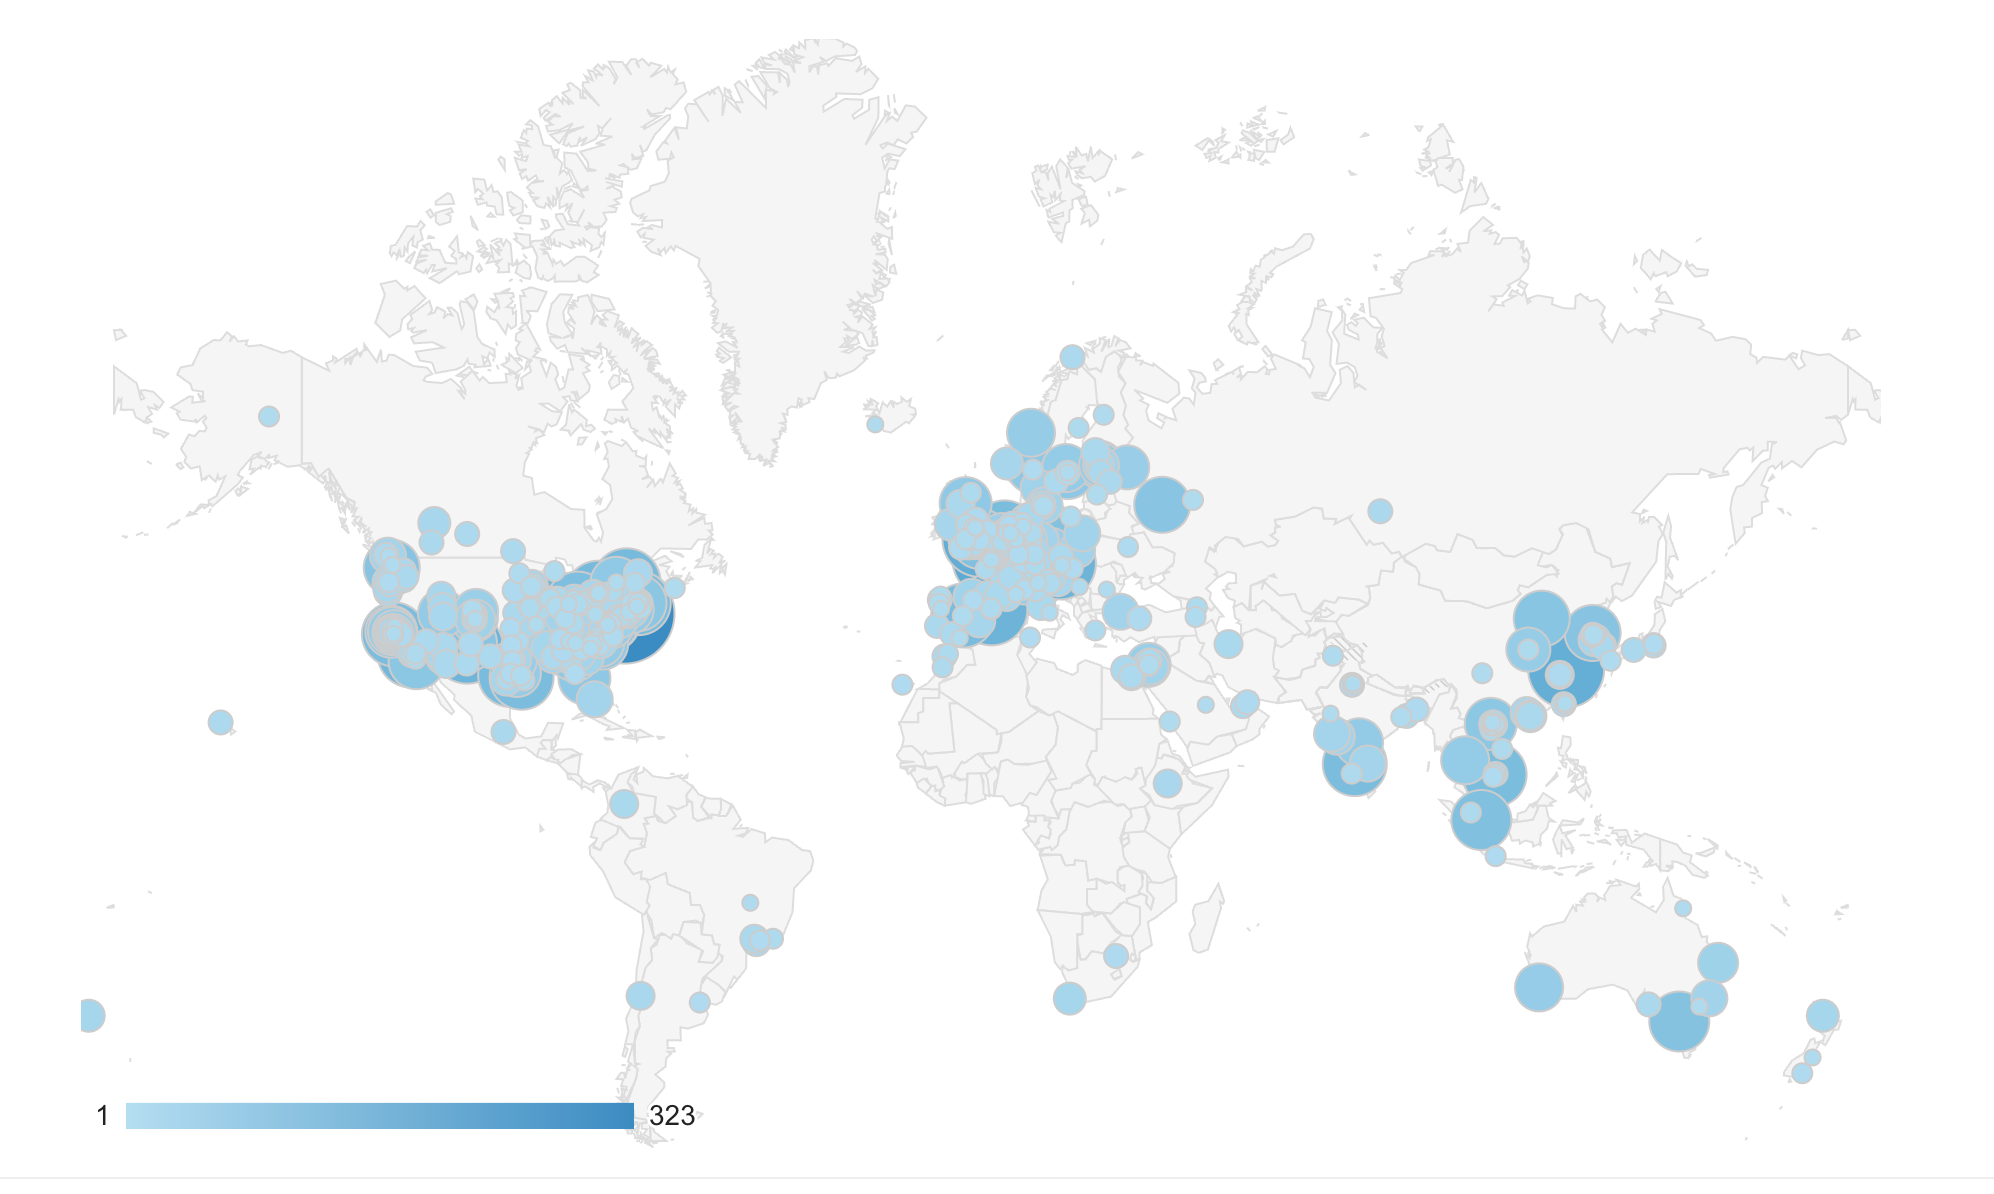
\includegraphics[width=.9\textwidth]{Lmod_doc_usage_by_city}}
\end{frame}

% page 20
\begin{frame}[fragile]
    \frametitle{Lmod Doc usage by Country}
    \center{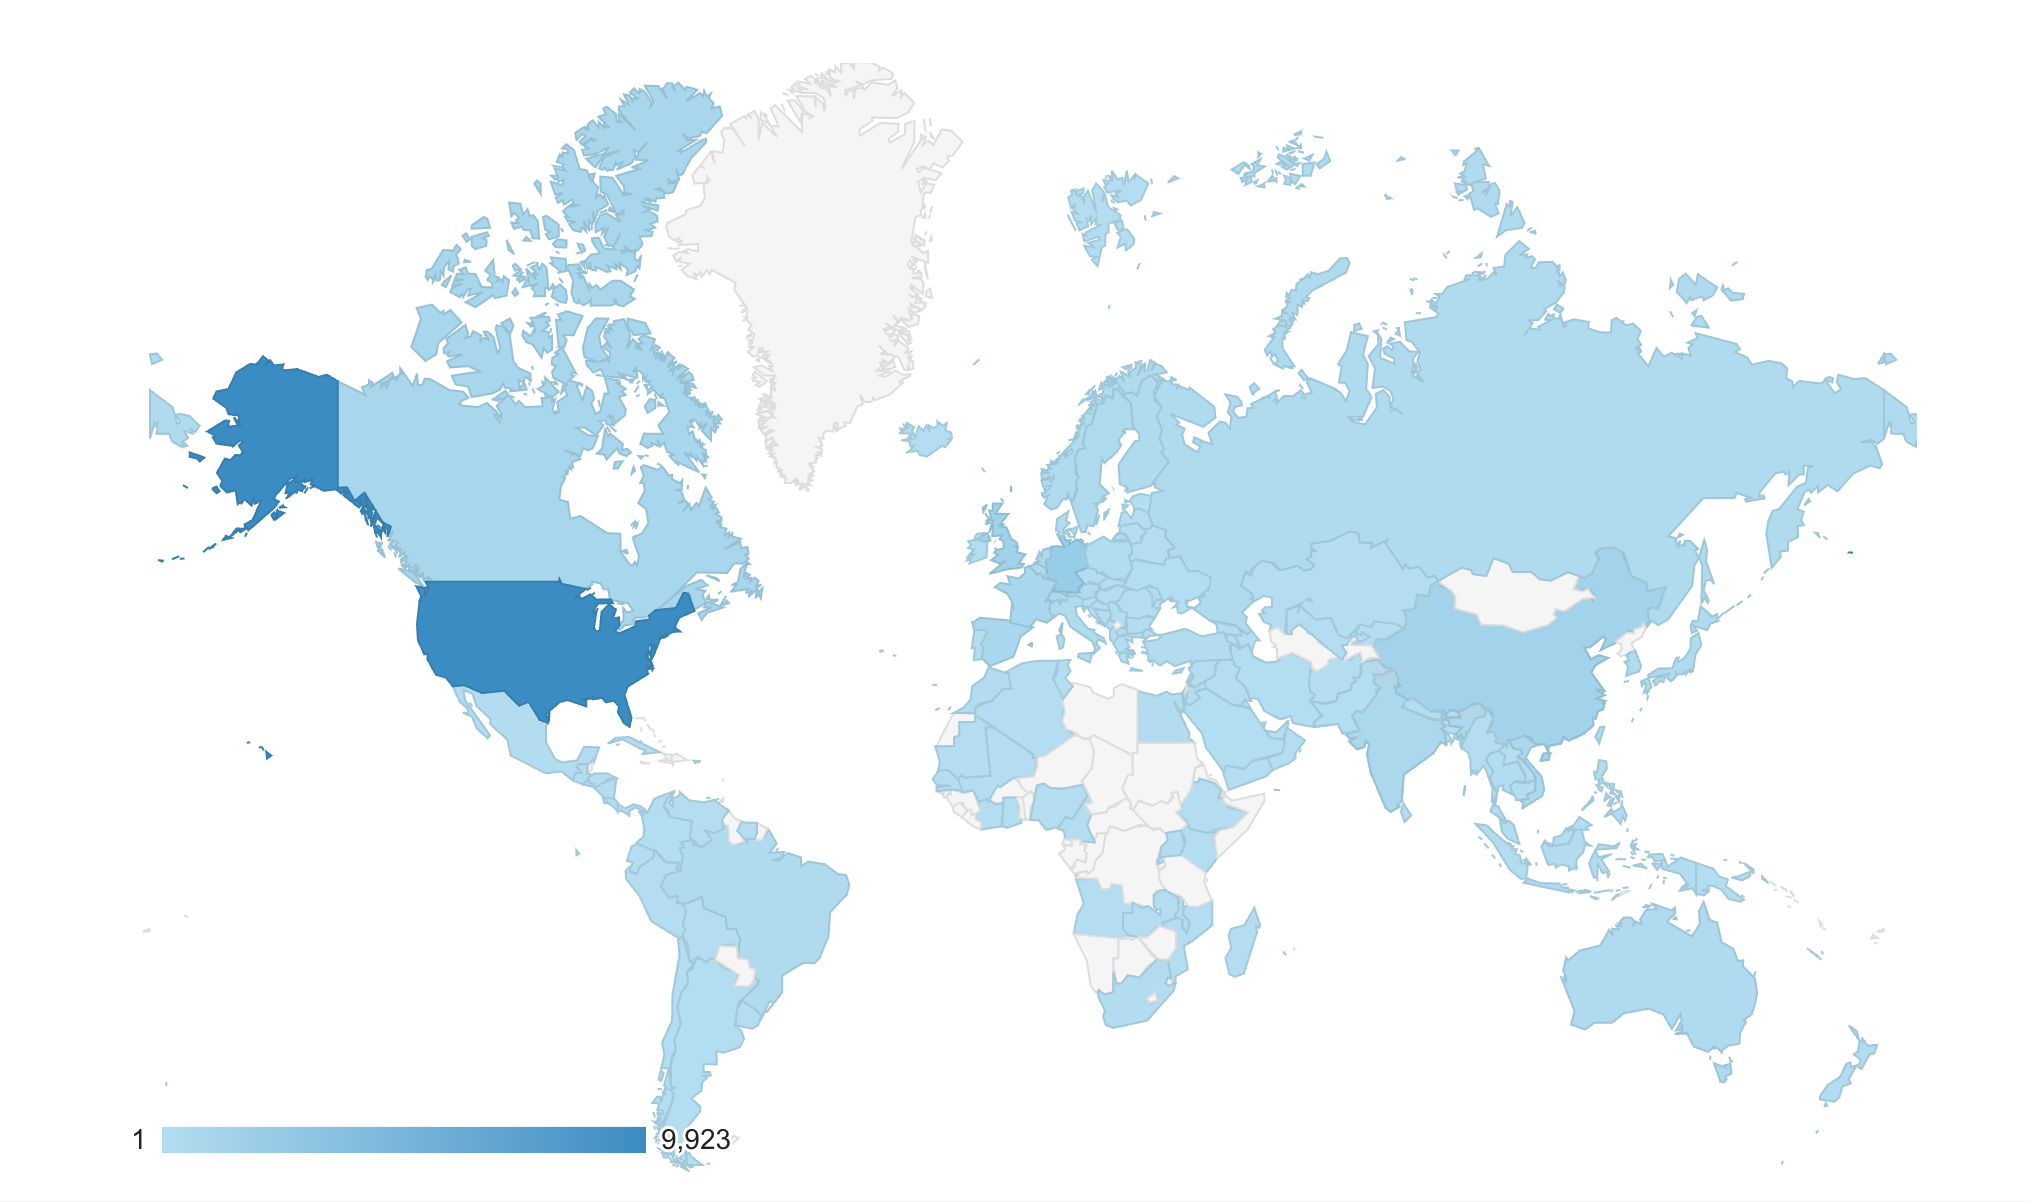
\includegraphics[width=.9\textwidth]{Lmod_doc_usage_by_country}}
\end{frame}

% page 21
\begin{frame}{Conclusions: Lmod 8+}
  \center{\includegraphics[width=.9\textwidth]{Lmod-4color@2x.png}}
  \begin{itemize}
    \item Latest version: https://github.com:TACC/lmod.git
    \item Stable version: http://lmod.sf.net
    \item Documentation:  http://lmod.readthedocs.org
    \item Talks:          https://github.com/TACC/lmod/tree/main/my\_docs/22
  \end{itemize}
\end{frame}

\end{document}
